\documentclass[a4paper]{article}
\usepackage{color}
\usepackage{url}
\usepackage[T2A]{fontenc}
\usepackage[utf8]{inputenc} 
\usepackage{graphicx}
\usepackage{multirow}
\usepackage[english,serbian]{babel}
\usepackage[unicode]{hyperref}
\hypersetup{colorlinks,citecolor=red,filecolor=green,linkcolor=blue,urlcolor=blue}
\newtheorem{primer}{Primer}[section]

\begin{document}

\title{Moralna i etička dilema autonomnih vozila\\ \small{Seminarski rad u okviru kursa\\Računarstvo i društvo\\ Matematički fakultet}}



\author{Marija Božić\\mi18241@alas.matf.bg.ac.rs}
\date{16. septembar 2022.}
\maketitle


\abstract Ovaj rad se bavi odgovorom na pitanje: ,,Da li je etično proizvoditi autonomna vozila čiji će izbor uticati na život vozača i okoline?'' Iznijete su činjenice zašto su ova vozila etički ispravna, kao i  činjenice koje su protiv proizvodnje ovih automobila. Nakon analiziranja obje
strane, zaključiću rad svojim odgovorom na ovo pitanje.

\tableofcontents
\newpage

\section{Uvod}
\label{sec:uvod}
\indent~Problem trolejbusa je misaoni eksperiment u etici. U opstoj formi problem glasi: Postoji trolejbus koji nema kontrolu nad svojim funkcijama i kreće prema petoro ljudi koji su zavezani na šinama. Ti stojiš pored poluge koja može da preusmjeri trolejbus u drugu traku. Ako povučeš polugu trolejbus će promjeniti traku i pet ljudi koji se nalaze na glavnoj traci će biti spašeno.\\
Međutim na sporednoj traci leži jedna osoba. Imaš dvije opcije:
\begin{enumerate}
\item~Ne uraditi ništa i dozvoliti da trolejbus ubije pet ljudi na glavnoj traci.
\item~Povući polugu i preusmjeriti trolejbus na sporednu traku i tako ubiti jednog čovjeka.
\end{enumerate}
Koja opcija je etički ispravna?
\begin{figure}[!h]
\begin{center}

\includegraphics[scale=0.3]{1.png}
\label{1}
\caption{Problem trolejbusa}
\end{center}
\end{figure}\\
\indent~Danas se ovaj problem često javlja u diskusiji o etici dizajna autonomnih vozila.
\vspace{0.2cm}\\
\indent~Autonomna vozila su jedna od tehnološki najnaprednijih inovacija koje je čovjek stvorio do danas. Kao i kod svake nove tehnologije pojavljuju se i nova etička pitanja koja je okružuju. Šta se dešava ukoliko vozilo mora da napravi izbor i presudi da li će u slučaju udesa povrijediti svog vlasnika ili druge učesnike u saobraćaju?\\  Sa ubrzanim razvojem autonomnih vozila, rješenje ove psihološke i socijalne dileme želi da čuje sve veći broj budućih kupaca. Drugim riječima, ljudi žele da kao vlasnici ovih automobila zaštite pješake i vlasnike drugih automobila, ali ne žele da odustanu od svoje bezbjednosti.\cite{7}
\vspace{0.2cm}\\
\indent~Tim istraživača sa Univerziteta u Kaliforniji na čelu sa profesorom psihologije Azimom Sarifom, sproveo je istraživanje javnog mnjenja po pitanju nekoliko hipotetičkih scenarija koji se mogu dogoditi. Jedan od njih je bio kakvu odluku robot treba donijeti u situaciji kada postoji opasnost da auto naleti na grupu neopreznih pješaka?  Koju etičku odluku će donijeti, ako je jedina opcija da se zakuca u zid ili padne niz liticu u pokušaju da sačuva njihove živote?\\  Kada su suočeni sa ovakvom dilemom, budućim kupcima malo znače uvjeravanja proizvođača, zasnovana na opštoj statistici, koji tvrde da se ogroman broj smrtnih ishoda i povreda izazvanih ljudskim faktorom može izbjeći upotrebom autonomnih vozila koja se oslanjaju na najsavremenije senzore i sisteme kontrole bezbjednosti. Tim istraživača je pokrenuo  sajt  Moral Machine ({\href{https://www.moralmachine.net/}{https://www.moralmachine.net/}), gdje se ova tehnološka i moralna pitanja dublje analiziraju kroz interaktivnu komunikaciju sa posjetiocima.

\section{Očekivanja i vrijednosti zainteresovanih strana}
\label{sec:očekivanja i vrijednosti zainteresovanih strana}
\begin{description}
\item~{\textbf{Ljubitelji autonomnih vozila}}\\Njihovo očekivanje je da budu u stanju da koriste ova vozila kako bi ih dovezla od tačke A do tačke B. Oni cijene inovaciju, efikasnost, pouzdanost i bezbjednost ovih vozila.
\item~{\textbf{Kompanije koje proizvode ova vozila (Tesla i Google)}}\\Njihova očekivanja su da budu u stanju da pruže uslugu koju zahtjevaju pomenuti ljubitelji ovih vozila. Oni cijene otvorenost društva prema stvaranju autonomnih vozila, slobodu inovacija i stalnu
podršku zainteresovanih ljudi.
\item~{\textbf{Posmatrči}}\\Njihovo očekivanje je da im ovi automobili ne naude kada putuju. Oni vjeruju da je društvena
odgovornost kompanija i vlade da brinu o bezbjednosti i dobrobiti svih posmatrača i učesnika u saobraćaju.
\item~{\textbf{Vlada i kreatori politike}}\\Njihovo očekivanje je da unaprijede društvo stvaranjem pravila i propisa za nove inovacije,
minimiziranjem rizika i zaštite građana. Oni cijene sigurnost, efikasnost i produktivnost.
\end{description}

\section{Autonomna vozila su etički ispravna}
\label{sec:autonomna vozila su etički ispravna}
\subsection{Algoritmi su pametni i kreirani od strane \\najstručnijih ljudi}
\label{subsec:algoritmi su pametni i kreirani od strane najstručnijih ljudi}
\indent~U djelu ,,Self-driving cars make ethical choices'', Nelson objašnjava složeni algoritam koji su Google i slične kompanije izgradile za kreiranje autonomnih vozila.\cite{6} Proces izrade softvera nije bio jednostavan i zahtjevao je najpametnije ljude širom svijeta. Na kraju krajeva, Google-ova stopa zapošljavanja je oko $0,2\%$  (Eadicicco).\cite{4} Poznato je da ove kompanije zapošljavaju ne samo najprestižnije kandidate sa odgovarajućim vještinama, već  i najetičnije svjetske pojedince.\\Izgradnja autonomnih vozila zahtjevala je mnogo godina istraživanja, razvoja i saradnje između više funkcionalnih timova, pošto je svaki detalj pažljivo proučavan i testiran. Algoritmi se kontinuirano uče, a poboljšanja se stalno vrše kako bi se usavršila tehnologija autonomnih vozila.
\vspace{0.2cm}\\
\indent~Nelson objašnjava kako funkcioniše Google-ov algoritam za samostalno upravljanje. Kada autonomno vozilo vidi biciklistu, malo bi se pomjerilo u svojoj traci da bi biciklista dobio više  prostora. Google-ov algoritam izračunava vjerovatnoću prema veličini rizika, upoređuje je sa vrijednošću informacija koje treba dobiti i koristi ih za donošenje odluka. Ako vas kamion udari sa strane, rizik od toga je $5.000$, udes u direktnom sudaru sa drugim automobilom ima magnitudu rizika od $20.000$, a udaranje pješaka ima magnitudu rizika od $100.000$. Ovaj sistem bodova izračunava vrijednost za različite scenarije, ljude, životinje, objekte i donosi brze odluke za najbolji način djelovanja.
\vspace{0.2cm}\\
\indent~Vožnja će uvijek uključivati rizik za različite strane, a Google je podjelio svoje gledište o etičkom procesu donošenja odluka raspodjelom rizika među stranama. Google vjeruje da autonomna vozila mogu donijeti etičke odluke ako ih inženjeri programiraju da uče i izračunavaju vrijednost situacija iz stvarnog života. Algoritmi koje je razvio Google i slične kompanije sadrže godine razmišljanja i istraživanja vrhunskih mislilaca u svijetu. Stoga, mnogi mogu trvditi da to opravdava slučaj za korišćenje autonomnih vozila.

\subsection{Autonomna vozila su bezbjednija od \\automobila kojima upravljaju ljudi}
\label{subsec:autonomna vozila su bezbjednija od automobila kojima upravljaju ljudi}
\indent~Dokazi pokazuju da će ovi automobili dramatično smanjiti saobraćajne nesreće, do $90\%$, sprijeciti do $190$  milijardi dolara štete i zdravstvenih troškova godišnje i spasiti hiljade života.\cite{1} Ovi automobili su programirani da poštuju sve saobraćajne zakone. Njih tokom vožnje ne ometaju mobilni telefoni, niti voze pijani ili zaspe. Oni su odlični u otkrivanju i izbjegavanju prepreka i imaju jaču oštrinu  vida od ljudskog oka. Imaju pogled na okolinu od $360^{\circ}$ i mogu da obrađuju znatno više informacija od običnog čovjeka.\\ \indent Istraživanja pokazuju da su saobraćajne nesreće mnogo rjeđe, a da  ljudi imaju negativnu percepciju zbog medija koji uglavnom preuveličavaju situaciju.\cite{2} Kada su ljudi umješani u saobraćajnu nesreću, lako je oprostiti, jer znamo da ljudi instiktivno štite sebe u tim trenucima. Međutim, ljudi nemaju isti način razmisljanja kada su u pitanju autonomna vozila, jer ona ne reaguju, ona su isprogramirana da izvode određene radnje. Iako postoje jasni dokazi da su autonomna vozila mnogo bezbjednija od automobila kojima upravljaju ljudi, većina je i dalje zaslijepljena sa nekoliko saobraćajnih nesreća koje su se dogodile ovim automobilima.

\subsection{Autonomna vozila će učiniti svijet boljim \\mjestom}
\label{subsec:autonomna vozila će učiniti svijet boljim mjestom}
\begin{figure}[h!]
\begin{center}
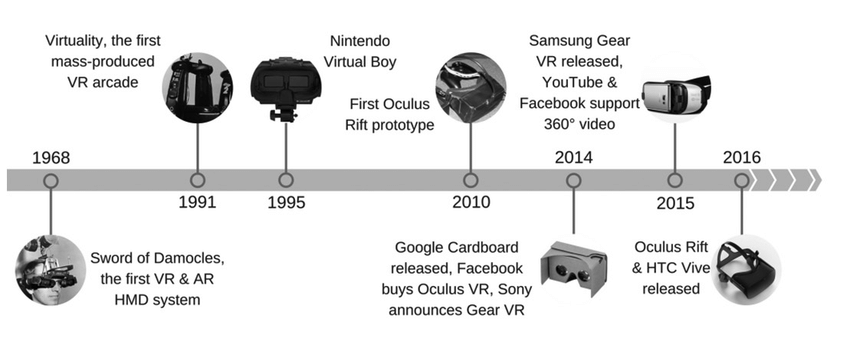
\includegraphics[scale=0.4]{2.png}
\label{2}
\caption{Sigurna i produktivna vožnja u autonomnom vozilu}
\end{center}
\end{figure}\\
\indent~Ovi automobili mogu poboljšati svačiji način života. Takođe utiču na smanjenje gužve u saobraćaju.\cite{3} Pomažu da se obezbjedi kretanje konstantnom brzinom. Pošto su saobraćaj i saobraćajne gužve glavni problem za gradove, ovo je jedan od važnih razloga da se odobri i opravda upotreba ovih vozila.\\  
\indent Kod ovih vozila je takođe minimizovana potrošnja goriva. Uprava za energetske informacije je predvidjela da bi do $2050$. godine ova vozila mogla da smanje potrošnju goriva za $44\%$ za automobile i $18\%$ za kamione. Američko transportno društvo predviđa da bi ovi automobili mogli dovesti do smanjenja potrosnje nafte za $2-4\%$.\cite{5} Na kraju, ovi automobili mogu smanjiti neproduktivno i stresno vrijeme vožnje. Ljudi će za vrijeme vožnje moći da jedu, spavaju ili obavljaju neke druge zadatke dok automobil vozi. Ovo je posebno bitno ljudima koji putuju na posao i svakodnevno provode u automobilu više od dva sata.

\section{Autonomna vozila nisu etički ispravna}
\label{sec:autonomna vozila nisu etički ispravna}
\subsection{Slučajne\, oduke su bolje od unaprijed određenih}
\label{subsec:slučajne oduke su bolje od unaprijed određenih}
\indent~Ljudi mogu tvrditi da su slučajne ljudske nesreće opravdanije od algoritma koji je već unaprijed odredio smrt nekog u saobraćajnoj nesreći. Pored ovoga mnogi se pitaju ko bi snosio odgovornost za izazvanu nesreću. Da li je odgovornost vozača, proizvođača automobila, ili inženjera koji je razvio softver. Mnogi vjeruju da je situacija previše složena i da ljudi treba da dozvole da se nesreće dešavaju prirodno. Drugi misle da nije etički ispravno da ljudi donose odluke o životu druge osobe i favorizuju slučajne nesreće.\\
\indent Na Univerzitetu u Bolonji vršena su istraživanja šta bi se dogodilo kada bi vozač ipak imao kontrolu u nekoj mjeri. Tim je dizajnirao brojčanik koji će omogućiti vozačima da izaberu jednu od 3 opcije voznje: altruistično, potpuno egoistično ili nepristrasno. Automobil će uzeti znanje koje mu pruža vozač i u zavisnosti od toga izvršiti unaprijed određenu radnju.\\
\begin{figure}[h!]
\begin{center}
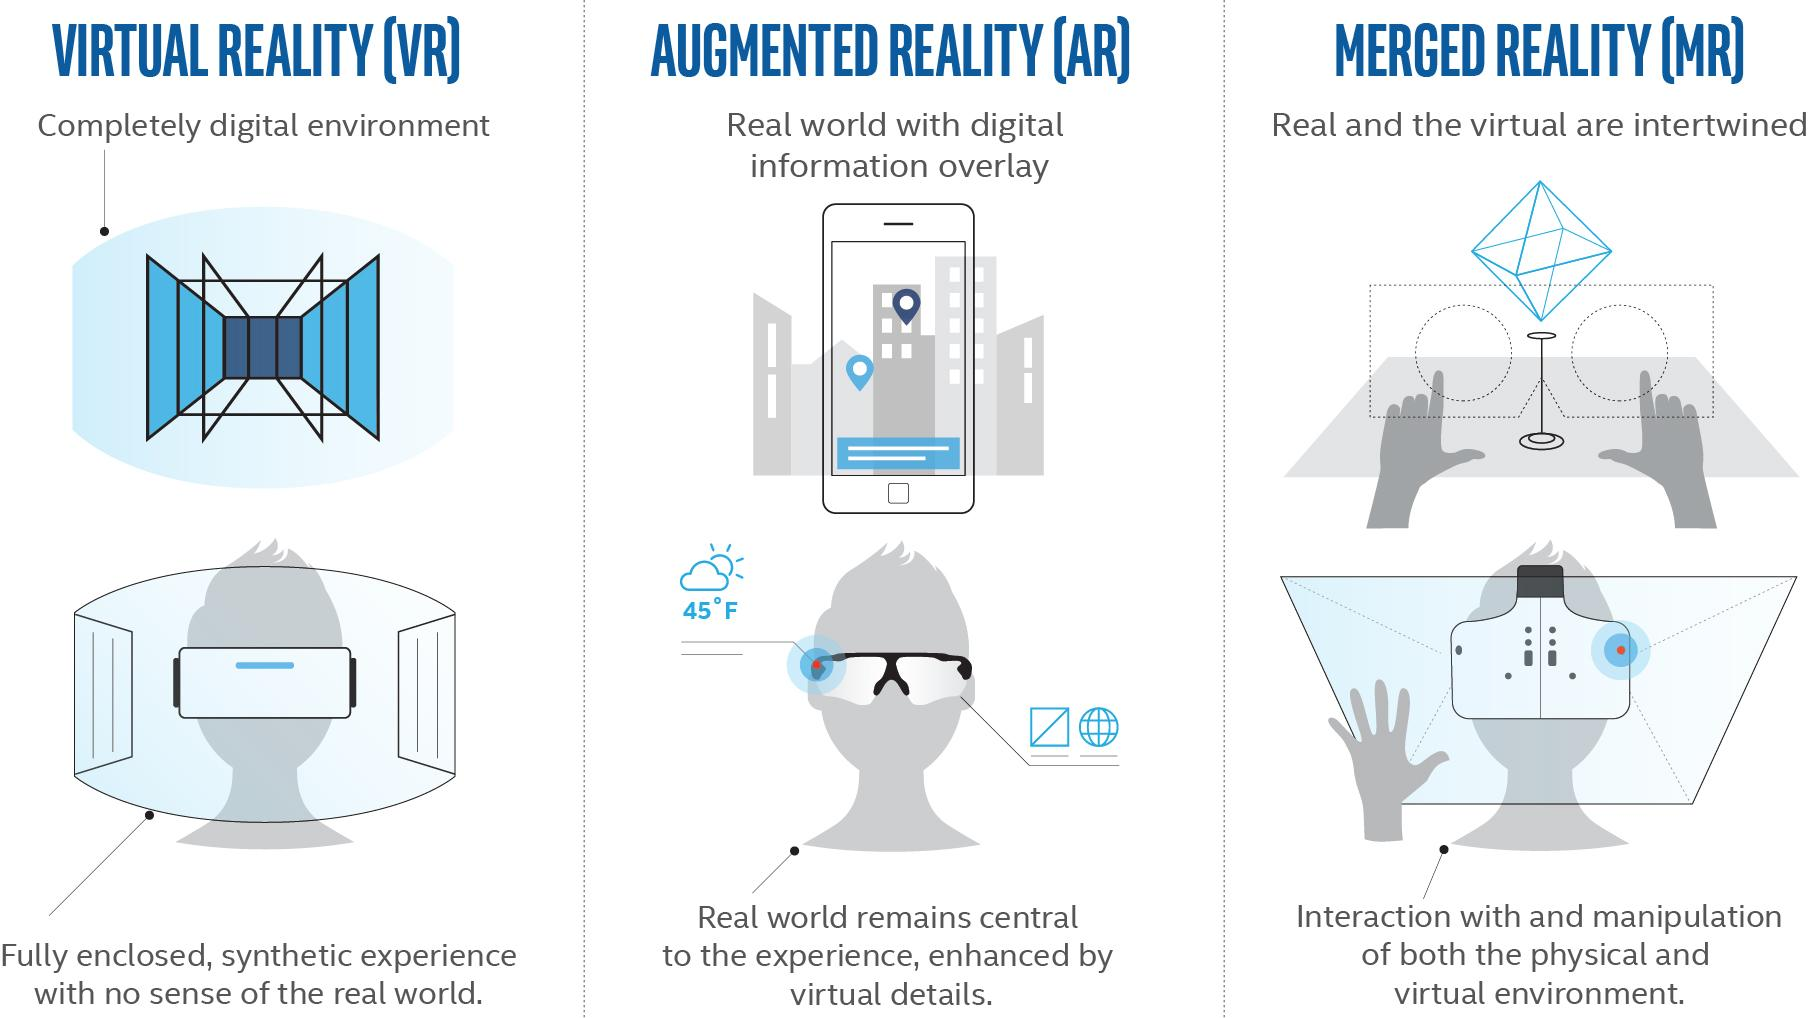
\includegraphics[scale=0.37]{3.png}
\label{3}
\caption{Donošenje etičkih odluka: Zaštiti sebe ili druge?}
\end{center}
\end{figure}\\
\indent  Ali, glavna etička pitanja i dalje nisu rješena. Šta ako bi svi izabrali nepristrasnu vožnju, ili svi izabrali egoističnu? Ovo rješenje je dalo ljudima određenu kontrolu nad njihovim autonomnim vozilima, ali samo u određenoj mjeri, ostavljajući glavna etička pitanja i dalje nerješenim.

\subsection{Ne bismo trebali da dozvolimo kompanijama, vladama i kreatorima politike da kontrolišu našu sudbinu}
\label{subsec:ne bismo trebali da dozvolimo kompanijama, vladama i kreatorima politike da kontrolišu našu sudbinu}
\indent~Ljudi mogu da tvrde da je neetično da neko osim njih samih odlučuje o njihovoj sudbini. U slučaju ovih vozila, inženjeri su razvili tehnologiju na osnovu svoje etike. Kreatori politike i vlada takođe pokušavaju da postave pravila i propise o autonomnim vozilima. Njemačka je pokušala da riješi etička pitanja autonomnih vozila stvarnim smjernicama. Nacija je predložila da autonomna vozila uvijek treba da pokušaju da izbjegnu ili minimizuju ljudsku smrt i ne bi trebalo da prave razliku između pojedinaca na osnovu starosti, pola ili bilo kog drugog faktora. Takođe su predložili da ljudskim životima treba dati prioritet nad životinjama ili imovinom. Prema studiji  $75\%$  učesnika je podržalo ovaj pristup, a $25\%$  je bilo protiv.

\subsection{Skladište podataka i hakeri predstavljaju\\ prijetnju za društvo}
\label{subsec:skladište podataka i hakeri predstavljaju prijetnju za društvo}
\indent~Ogromna količina podataka mora da se prikupi preko senzora, kako bi ova vozila ispravno radila. Dok voze ovi automobili neprekidno čuvaju podatke o svom okruženju, koja im omogućavaju da uče i postanu pametniji. Ovo postavlja mnoga bezbjednosna pitanja, jer ovi automobili drže velike količine podataka, uključujući gdje su bili vozač i suvozač, razgovore u vozilu, komunikaciju putem mobilnih telefona. Zloupotreba ovih podataka može biti štetna za identitet, finansije  i egzistenciju osobe.\\
\indent Takođe postoji velika bojazan da će kriminalci da hakuju i upravljaju automobilima na daljinu.
\begin{figure}[!h]
\begin{center}
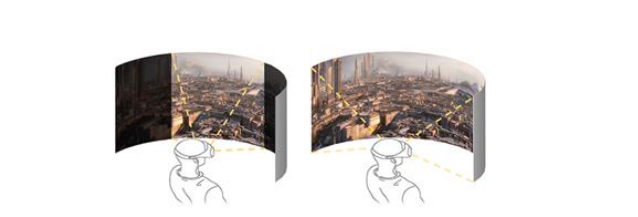
\includegraphics[scale=0.85]{4.jpeg}
\label{1.1}
\caption{Haker}
\end{center}
\end{figure}
\newpage
\section{Zaključak}
\label{sec:zaključak}
\indent~Utilitarizam autonomnih vozila je energično i branjen i napadan. Kada ljudi sjednu na mjesto vozača, zakon kaže da oni preuzimaju punu odgovornost za svoje postupke. Kada su u pitanju atonomna vozila, postoji jasna siva zona: da li je vozač odgovoran za bilo kakvu štetu nanijetu nedužnim prolaznicima koji su povrijeđeni od strane autonomnih vozila? Ili je automobil odgovoran za štetu? Ljudi i autonomna vozila koji dođu u situaciju neizbježne nesreće moraju u djeliću sekunde da donesu moralne odluke o tome da li da zaštite sebe ili druge.\\
\indent Zbog sive zone bilo je mnogo debata o tome da li su ovi automobili etički ispravni.
\vspace{0.2cm}\\
\indent~Ja bih prednost dala pozitivnim stranama. Ove automobile kreiraju neki od najinovativnijih i najobrazovanijih ljudi današnjeg društva. Pored toga, ovi automobili su se pokazali znatno bezbjednijim od stvarnog vozača; to su pokazale brojne studije i prikupljeni podaci. Dugoročno gledano, ovi automobili će povećati efikasnost i produktivnost za ljude širom svijeta. Da bi se više ljudi osjećalo opušteno u autonomnim vozilima, kompanije treba da shvate da su odgovorne za bezbjednost svih zainteresovanih strana. Tehnike upravljanja rizikom se mogu koristiti za kvantifikaciju vjerovatnog rizika na način koji je transparentan i fleksibilan. Da bi stvorili etička sredstva, programeri bi trebalo da nastave da uče iz prošlih iskustava u upravljanju rizikom i moralno izazovnih situacija.\\
\indent Kako nauka i tehnologija napreduju neizbježno je da će se razvijati više izuma. Ljudi samo trebaju da ne odustaju od propisa kojima bi sebe zaštitili. 

\newpage
\addcontentsline{toc}{section}{Literatura}
\begin{thebibliography}{99}
\bibitem{1}Beall, A. (October 18, 2017). The car you can program to sacrifice you in crash. New Scientist. Retrieved from Nexis Uni.
\bibitem{2}Bohn, D. (2016, October 20). Elon Musk: Negative media coverage of autonomous vehicles could be ‘killing people’. Retrieved from {\href{https://www.theverge.com/2016/10/19/13341306/elon-musknegative-media-autonomous-vehicles-killing-people}{https://www.theverge.com/2016/10/19/13341306/elon-musknegative-media-autonomous-vehicles-killing-people}}
\bibitem{3}Brown, D. (2018, July 04). How self-driving car or adaptive cruise control could ease traffic jams. Retrieved from {\href{https://www.usatoday.com/story/money/2018/07/03/selfdriving-
reduces-traffic-jams-study-says/741985002/}{https://www.usatoday.com/story/money/2018/07/03/selfdriving-
reduces-traffic-jams-study-says/741985002/}}
\bibitem{4}Eadicicco, L.\,(2014, October 23).\,Here’s Why You Probably Won’t Get Hired At Google. Retrieved from\\ {\href{https://www.businessinsider.com/google-hiring-processcommittee-2014-10}{https://www.businessinsider.com/google-hiring-processcommittee-
2014-10}}
\bibitem{5}Pyper, J. (2014, September 15). Self-Driving Cars Could Cut Greenhouse Gas Pollution. Retrieved from\\
{\href{https://www.scientificamerican.com/article/self-driving-cars-could-cut-greenhouse-gas-pollution/}{https://www.scientificamerican.com/article/self-driving-cars-could-cut-greenhouse-gas-pollution/}}
\bibitem{6}Nelson, G. (July 13, 2015). Self-driving cars make ethical choices. Automotive News Print Version. Retrieved from Nexis
Uni.
\bibitem{7}Trappl, R. (n.d.). Ethical Systems for Self-Driving Cars: An Introduction. Applied Artificial Intelligence, 30(8), 745–747.
{\href{https://doi.org/10.1080/08839514.2016.1229737}{https://doi.org/10.1080/08839514.2016.1229737}}
\end{thebibliography}
\end{document}